% Created 2024-09-02 Mon 18:52
% Intended LaTeX compiler: pdflatex
\documentclass[letterpaper, 12pt]{article}
\usepackage[utf8]{inputenc}
\usepackage[T1]{fontenc}
\usepackage{graphicx}
\usepackage{longtable}
\usepackage{wrapfig}
\usepackage{rotating}
\usepackage[normalem]{ulem}
\usepackage{amsmath}
\usepackage{amssymb}
\usepackage{capt-of}
\usepackage{hyperref}
\usepackage{minted}
\usepackage{xcolor}
\usepackage{hyperref}
\usepackage{tocloft}
\usepackage{minted}
\usemintedstyle{manni}
\usepackage{pdfpages}
\usepackage{fancyhdr}
\usepackage{graphicx}
\usepackage[top=1.4in, left=0.5in, right=0.5in, bottom=0.8in]{geometry}
\usepackage[T1]{fontenc}
\usepackage{helvet}
\pagestyle{fancy}
\renewcommand{\headrulewidth}{0pt}
\renewcommand{\footrulewidth}{0pt}
\setlength{\parindent}{0em}
\setlength{\parskip}{1em}
\usepackage{hyperref}
\usepackage {color}
\usepackage {tabularray}
\usepackage{xcolor}
\hypersetup{
colorlinks=true,
linkcolor=blue,
filecolor=magenta,
urlcolor=cyan,
citecolor=green,
pdfborder={0 0 0}
}
\usepackage[most]{tcolorbox}
\author{Hilduara Abreu}
\date{\today}
\title{PS192 | Missing Student Protocol\\\medskip
\large English Version}
\hypersetup{
 pdfauthor={Hilduara Abreu},
 pdftitle={PS192 | Missing Student Protocol},
 pdfkeywords={},
 pdfsubject={},
 pdfcreator={Emacs 29.4 (Org mode 9.6.15)}, 
 pdflang={English}}
\begin{document}

\fancyfoot[C]{\setlength{\unitlength}{1in}\begin{picture}(5,0)\put(-1.8,-0.5){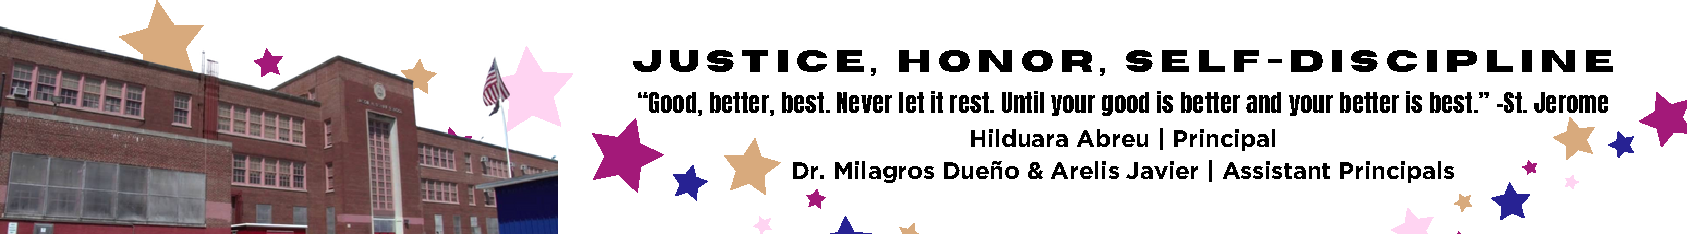
\includegraphics[width=8.8in,height=1.3in]{logo-1}}\end{picture}}
\fancyhead[C]{\setlength{\unitlength}{1in}\begin{picture}(5,0)\put(-1.9,-0.5){
\includegraphics[width=8.9in,height=1.3in]{logo-2}}\end{picture}}
\fancyhead[R]{\thepage}
\pagenumbering{gobble}

\begin{document}
\newpage
\vspace*{-0.3cm}

\textbf{Re: Implementation of the Missing Student Protocol, effective as of September 5th, 2024}

This Missing Student Protocol is established to ensure the safety and well-being of all students at PS192. It outlines the steps to be taken immediately if a student is identified as missing, ensuring a swift and efficient response by all staff members. The protocol aligns with NYCDOE and UFT guidelines and is designed to provide clarity and consistency in handling such critical situations.

\textbf{Reporting a Missing Child}

\begin{itemize}
\item \textbf{\textbf{Immediate Reporting}}: If a staff member identifies a missing child or notices a child who eludes adult supervision, they must immediately use their cell phone to text the administration and the parent coordinator while they are seeking or following the child.
\item \textbf{\textbf{Building Response Team (BRT) Activation}}: If the child is confirmed missing, the Principal will activate the Building Response Team (BRT) to assist in locating the student and preventing them from leaving the premises.
\end{itemize}

\textbf{Search Efforts}

\begin{itemize}
\item \textbf{\textbf{Comprehensive Search}}: The BRT and all available school staff will conduct a thorough search of both indoor and outdoor areas throughout the entire school premises.
\item \textbf{\textbf{Intercom Announcement}}: An announcement will be made via the school-wide intercom by the secretary, using the code phrase: "The lion is out of the den. Call me if you see him or find him." This alert notifies staff of the missing child and helps gather information on the student's last known location.
\item \textbf{\textbf{Law Enforcement Notification}}: If the child is not found within a specific timeframe, local law enforcement will be notified. The Principal and/or the BRT chairperson will be responsible for contacting 911 and informing the Borough Safety Director and the D6 Superintendent.
\item \textbf{\textbf{Student Information Profile}}: Upon the arrival of law enforcement, the Principal and/or BRT chairperson will provide them with a student information profile.
\end{itemize}

\textbf{Communication, Documentation, and Feedback}

\begin{itemize}
\item \textbf{\textbf{Parent/Guardian Notification}}: The administration will contact the parent or guardian to inform them of the situation. \newpage \vspace*{-0.5cm}
\item \textbf{\textbf{Incident Documentation}}: Staff members responsible for the child's supervision must complete an OORS report form detailing the incident before leaving the premises if the incident occurred before 1 p.m. The form will be submitted to Assistant Principal, Dr. Milagros Dueño.
\item \textbf{\textbf{Incident Review}}: The Principal will review the incident form with the UFT Chapter Leader and the BRT chairperson, gather feedback and suggestions, and may convene a meeting with the involved staff members for further review and discussion.
\end{itemize}

\textbf{Preventive Measures}

\begin{itemize}
\item \textbf{\textbf{Hallway and Bathroom Monitoring}}:
\begin{itemize}
\item \textbf{Second Floor}: Ms. Del Orbe, Ms. Cuesta, Mr. Abreu, and Mr. Suero oversee the monitoring of the second-floor hallway and bathrooms.
\item \textbf{First Floor}: Ms. Clemons, Ms. Rijo, and the designee assigned by the principal of MS 209 supervise the first-floor hallway and bathroom facilities.
\end{itemize}
\item \textbf{\textbf{Exit Security}}: Ms. Clemons, our safety agent, will consistently inspect and secure all exits to prevent unauthorized access.
\item \textbf{\textbf{Student Safety Education}}: During the SEL (Social-Emotional Learning) block, teachers will provide students with education on safety procedures and guidance on whom to contact if they feel lost or unsafe. This will occur once a month.
\end{itemize}

Your cooperation and strict adherence to this protocol and the preventive measures outlined are crucial to ensuring the safety and security of our students. By working together and maintaining vigilance, we can significantly contribute to the overall safety of our school environment.

Thank you for your attention and commitment to our students' safety.

With Justice, Honor, and Self-Discipline,


\includegraphics[width=0.16\textwidth]{hil_signature}

\textbf{Hilduara Abreu, Principal}

\textbf{The school of Joyful Learning!}

\href{www.ps192.org}{www.ps192.org}
\end{document}
